
\outline{3}{Exercise 12.9}
\subsubsection*{Exercise 12.9}

\textit{Estimate the critical percolation threshold for the same forest fire
model but with von Neumann neighborhoods. Confirm the analytical result by
conducting simulations.}

\vspace{5mm}
With von Neumann\textquotesingle s neighborhood, the system supports percolation
in the cases on the left side, and those on the right side are unsupported:
\begin{figure}[h]
  \centering
  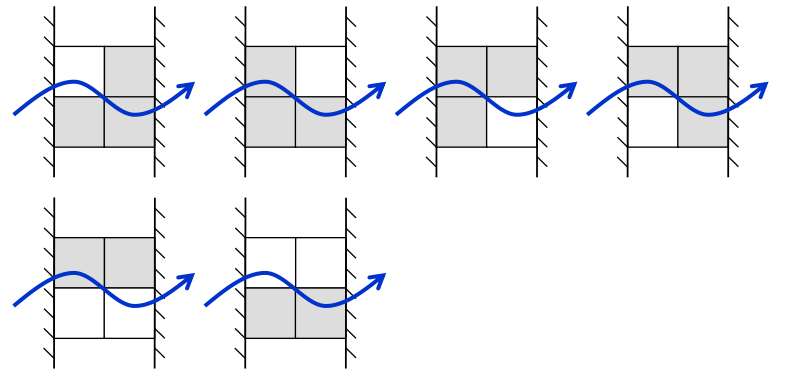
\includegraphics[width=0.5\textwidth]{./figures/12.9-supported-cases.png}
  \hspace{15mm}
  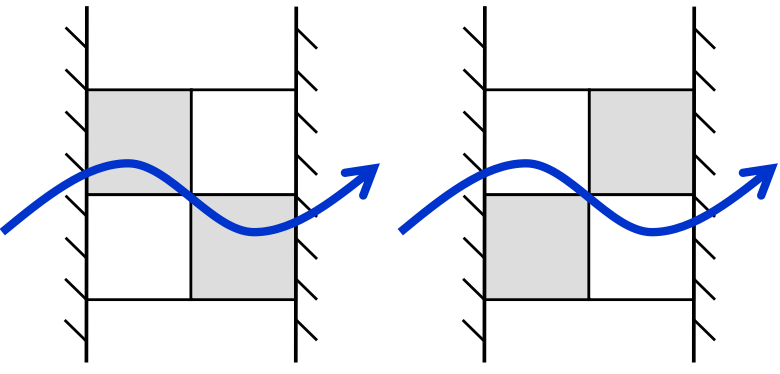
\includegraphics[width=0.25\textwidth]{./figures/12.9-unsupported-cases.png}
\end{figure}

So that the critical percolation threshold is now given by:
\begin{equation}
  p_c = {p_c}^4 + 4 {p_c}^3 (1-p_c) + 2 {p_c}^2 {(1-p_c)}^2,
\end{equation}

and the cobweb plot for that equation is:
\begin{figure}[h]
  \centering
  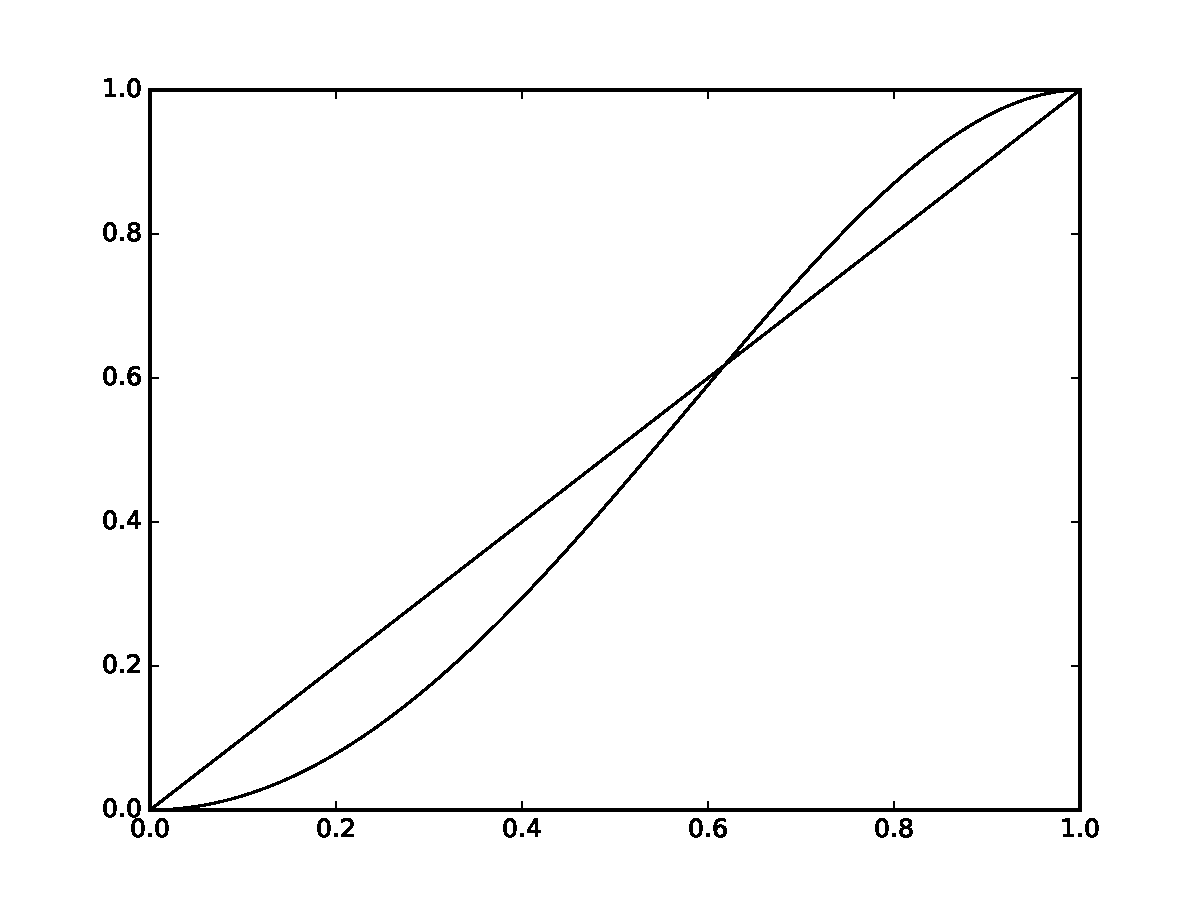
\includegraphics[width=0.75\textwidth]{./figures/12.9-cobweb-plot-for-von-neumann-neighborhood.pdf}
  \caption{\texttt{12.9-cobweb-plot-for-von-neumann-neighborhood.py}}
\end{figure}

In which is easy to see two asymptotic states possible, $p_\infty = 0$ and
$p_\infty = 1$ (the cobweb plot is about relations over scale, not about
dynamics over time). There is an unstable equilibrium point around $p = 0.6$.
The exact value is given by:
\begin{equation}
  p_c = \frac{\sqrt{5}}{2} - \frac{1}{2} \approx 0.6180.
\end{equation}

\vspace{5mm}
To verify this prediction, one could simulate the system a certain number of
times for each values of $p$.
\begin{itemize}
  \item $p > p_c$: systems should show percolation in most cases;
  \item $p < p_c$: systems should not show percolation in most cases;
  \item $p \approx p_c$: systems will show percolation in some cases.
\end{itemize}

The following figure is a simulation output for $n = 100$ and $p = 0.5875$:
\begin{figure}[h]
  \centering
  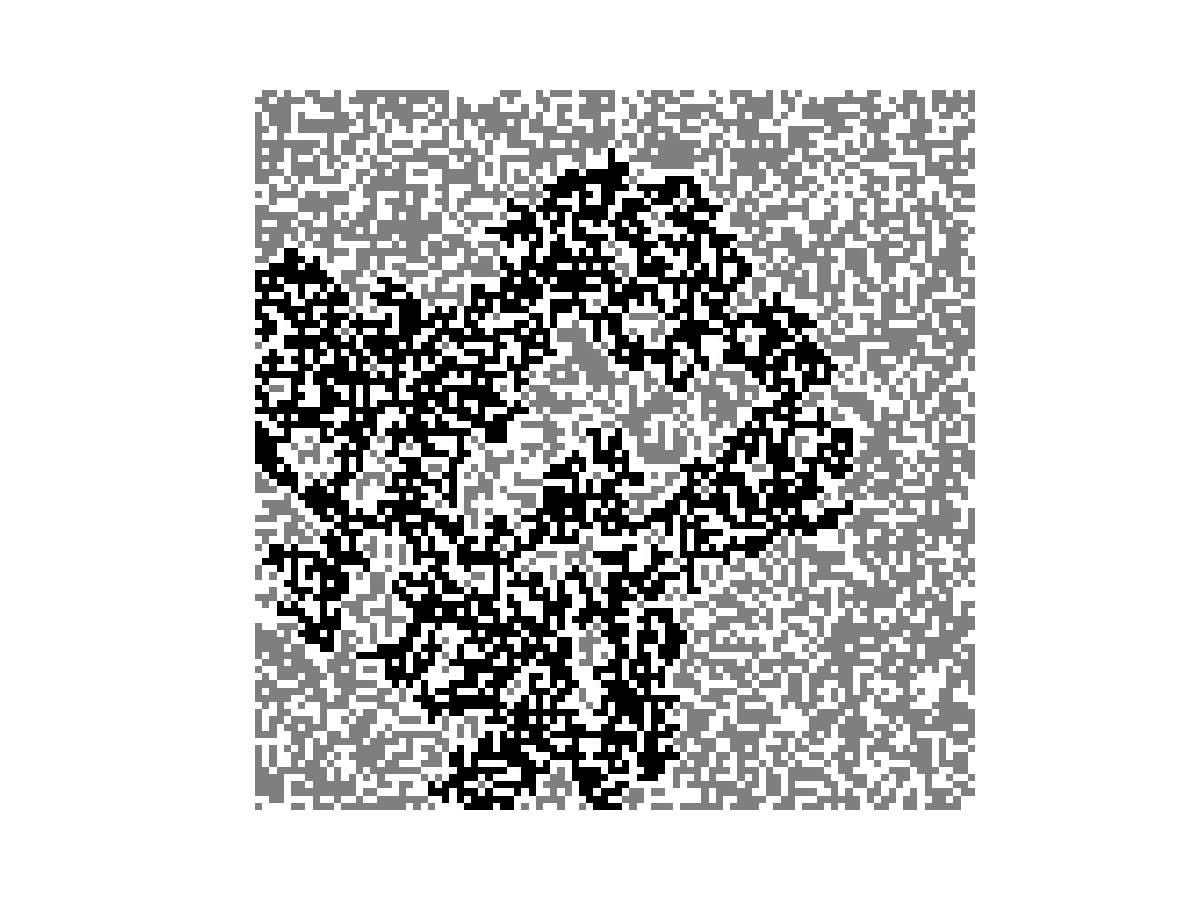
\includegraphics[width=0.75\textwidth]{./figures/12.9-simulation-result.pdf}
  \caption{\texttt{12.9-von-neumann-fire-ca.py}}
\end{figure}
